%%%%%%%%%%%%%%%%%%%%%%%%%%%%%%%%%%%%%%%%%%%%%%%%%%%%%%%%%%%%%%%%%%%%%%%%%%%%
\documentclass[a4j,dvipdfmx]{jarticle}

\usepackage{jsaisig}
\usepackage{amsmath}
\usepackage{graphicx}
\usepackage{calc,fancyvrb}
\usepackage{color}
\newcommand\mychangecolor[1]{\textcolor[rgb]{1,0,0}{\textbf{#1}}}
\usepackage{ascmac}
%%%%%%%%%%%%%%%%%%%%%%%%%%%%%%%%%%%%%%%%%%%%%%%%%%%%%%%%%%%%%%%%%%%%%%%%%%%

\begin{document}

%
\title{システム発話間の整合性を重視した発話選択への\\深層強化学習の適用}

%
\etitle{System Utterance Selection Considering Consistency between System Utterances with Deep Reinforcement Learning} 



\author{黒田 佑樹\afil{}%
	\thanks{連絡先: 大阪大学産業科学研究所\newline%
		 〒567-0047 大阪府茨木市美穂ケ丘8-1\newline%大阪大学産業科学研究所,大阪府茨木市美穂ケ丘8-1,06-6879-8416,akai@ei.sanken.osaka-u.ac.jp
		E-mail: y\_kuroda@ei.sanken.osaka-u.ac.jp}\quad%
    武田 龍\quad
	駒谷 和範\\
	Yuki Kuroda\afil{} \quad  Ryu Takeda\afil{}  \quad Kazunori Komatani}

%
\affiliation{%
	\afil{} 大阪大学 産業科学研究所\\ 
	\afil{} The Institute of Scientific and Industrial Research (SANKEN), Osaka University\\}


\abstract{
Our goal is to develop a listening-oriented dialogue system not by heavily depending on understanding results of user utterances but by simply controlling the sequence of system utterances. We previously implemented system utterance selection that considered consistency between the system's utterances using Q-learning. Deep Q-Network (DQN) can be used for taking more dialogue states into account. In this paper, we report our implementation of DQN to the same task. We used one-hot vectors as input representations of the dialogue states used in Q-learning and normalized rewards.  We conducted several text dialogues with the trained model and compared the number of dialogue breakdowns with our previous Q-learning model. We also compared the number of episodes required for the training.
}

%Abstract:ユーザ発話内容の解析に偏重することなく,システム発話の列をコントロールするだけで,聞き役の対話システムを実現することを目指している.我々は以前,システム発話の整合性を重視した発話選択を,Q学習を用いて実装した.さらにより多くの状態を考慮可能な強化学習を実装するために深層強化学習(DQN)を用いる.本稿では,以前実装したQ学習と同等の発話選択の実現を今回の目標として,深層強化学習を設計したので報告する.
%まず,Q学習で用いていた状態をone-hotベクトルを用いて入力表現とした.次に報酬として,これまで用いていたものを正規化して与えた. 評価としては,テキスト対話を行い,システム発話の破綻数を以前の手法と比較することで,同等の性能が再現できているかを調べた. 加えて,十分に学習できるまでのエピソード数の比較を行った.

\maketitle
\thispagestyle{empty}

%%%%%%%%%%%%%%%%%%%%%%%%%%%%%%%%%%%%%%

\section{はじめに}
近年,対話そのものを目的とする非タスク指向型の対話システムが盛んに研究されている.
本稿では,その中でもユーザの話の聞き役となるシステム\cite{meguro}\cite{ishida}に注目する.
聞き役の対話システムはユーザの話したい,聞いてほしいという欲求を満たすことが期待される.

我々は,システム発話の列をコントロールするだけで,聞き役の対話システムを実現することを目指している\cite{nishimoto}.
システム発話の選択においては,文脈的に不適切な発話を選択しないこと,また,ユーザをより満足させるような順序で選択することが重要となる.
我々は以前に,システム発話間の整合性に注目して,強化学習の手法の1つであるQ学習を行った\cite{kuroda}.


%対話においてユーザの満足度を高める際には,より多くの状態を考慮して発話選択を行いたい.%なぜ多くの状態を扱う必要があるのかが苦しい
%例えば,ユーザの表情や声色等の状態を強化学習に組み込めれば,よりユーザの状態に対応した発話選択を行うことができる.

今後より多くの状態を考慮して発話選択を行うために,行動価値関数をニューラルネットワークで近似する深層強化学習を導入する.
例えば,ユーザの表情や声色等からユーザの状態を推定し,これを強化学習に組み込めば,ユーザの状態に対応した発話選択が可能となる.


本稿では,深層強化学習の手法の1種であるDeep Q Network\cite{DQN_origin}(以下DQNと呼ぶ)を用いる.これによって当該タスクをDQNを用いて適切に学習させた.
また,Q学習を用いた場合とDQNを用いた場合で学習過程の変化を調べた.


%%%%%%%%%%%%%%%%%%%%%%%%%%%%%%%%%%%%%%

\section{システム発話間の整合性を重視した発話選択}\label{Qlearning_sekkei}
Q学習では,ある状態である行動をとる価値(Q値)が更新されていく.これは,あるターン$t$での状態$s_{t}$,行動$a_{t}$と,次のターン$t+1$での状態$s_{t+1}$,報酬$r_{t+1}$,また,学習率$\alpha$,割引率$\gamma$を用いて式\ref{Q}のように表される.
この行動価値関数は図\ref{Q_table}のようにQテーブルと呼ばれる表形式で表現される.
右辺の第2項が0となる理想のQ関数であり,これに近づくように学習が行われる.
\begin{equation}
\label{Q}
\begin{split}
&Q(s_{t+1},a_{t+1}) \\&= Q(s_t,a_t)+\alpha(r_{t+1}+\gamma*max_aQ(s_{t+1},a)-Q(s_t,a_t))
\end{split}
\end{equation}

我々の以前の研究では,システム発話やユーザ発話の特徴を状態として表現し,選択されたシステム発話に応じて人手で設計した報酬を与えていくことで,適切なシステム発話選択ができるような行動価値関数を求めた.

まず状態として,
\begin{description}\item{\emph{状態1: }}システム発話の対話行為\item{\emph{状態2: }}ユーザ発話内の特定名詞の有無\item{\emph{状態3: } }システム発話ID\end{description}
の3つを定義し,学習時には発話選択の直前のシステム発話とユーザ発話からこれらの状態を取得する.

次に,行動として選択されたシステム発話から,
\begin{description}\item{\emph{情報1: }}システム発話の対話行為\item{\emph{情報2: }}システム発話内の指示語の有無\item{\emph{情報3: }}システム発話ID\end{description}
の3つの情報を取得し,図\ref{Qlearning}のように状態と照らし合わせて報酬を与える.

ここで報酬を与える基準として,「対話行為の整合性」,「指示語の整合性」,「発話内容の整合性」の3点を考える.

「対話行為の整合性」に関しては,連続するシステム発話の対話行為の順番に報酬を与える.
例えばシステムが質問をすると,ユーザが何らかの応答を返すことが予想される.
この時,システムはすぐ次の質問をするより,何らかの反応(応答)を返した方が良いというような関係を決めておき,それに従って報酬を与えた.

「指示語の整合性」に関しては,システム発話内に指示語がある場合,その指示語が指す内容がユーザ発話に存在するかを確認する.
システム発話内に指示語があるのに,直前のユーザ発話に指示語が指す内容(特定名詞)が存在しない場合,負の報酬をつけた.

「発話内容の整合性」に関しては,直前のシステム発話から予想されるユーザ発話と噛み合わないシステム発話の選択を防ぎたい.
例えば,図\ref{hutekisetsu}のように,「競技は何をご覧になりますか」のような質問には,ユーザは何らかの競技を答えると予想できる.それに対する,システムの「それは大変ですよね」といったような食い違った反応の発話選択は不適切である.
これを防ぐため,内容的に食い違う発話IDの組み合わせを人手で記述したblacklistを用意しておいて,学習時にblacklistに該当するような発話の組み合わせが選択されたら,負の報酬を付けた.

また,ここまでの3つの状態は言語情報のみを用いた適切な発話選択のためのものであったが,それ以外に,最低限のユーザ満足度の考慮のために,ユーザが対話を楽しんでいるかどうかを表す
\begin{description}\item{\emph{状態4: }}ユーザ心象\end{description}
も状態として加えた.ここでは単純に,ユーザから入力された心象の高低に応じて報酬をつけた.さらに連続して高低が続く場合にはより大きな報酬をつけた.






\begin{figure}[tb]
    \centering
    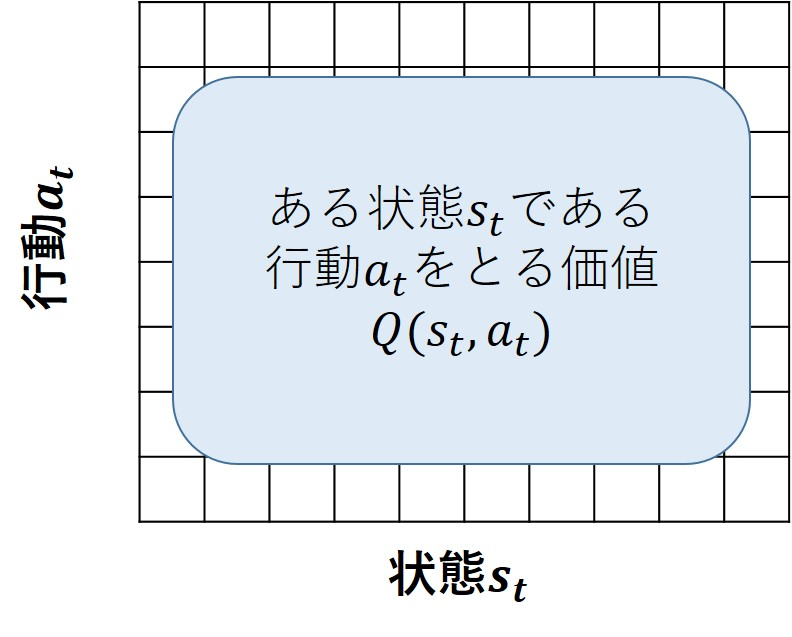
\includegraphics[width=0.5\hsize]{Q_table.jpg}
    \caption{Q学習の行動価値関数}
    \label{Q_table}
\end{figure}

\begin{figure}[tb]
    \centering
    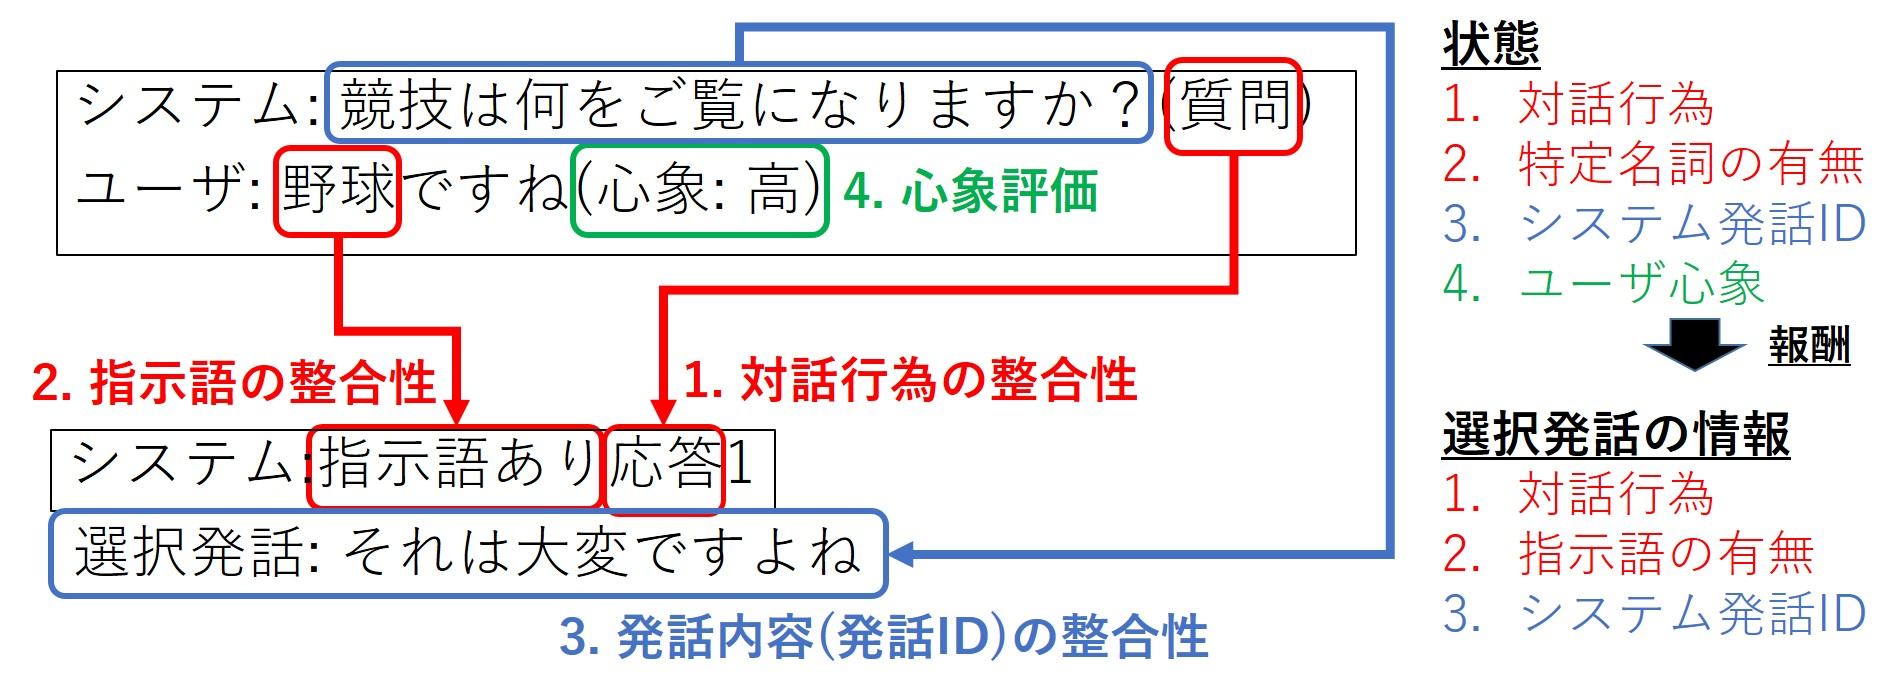
\includegraphics[width=\linewidth]{slud_Qlearning_re3.jpg}
    \caption{整合性を考慮する上で注目する関係}
    \label{Qlearning}
\end{figure}



\begin{figure}[tb]
\begin{screen}
\begin{Verbatim}[commandchars=\\\{\}]
S: 競技は何をご覧になりますか?
U: 野球です
\mychangecolor{S: それは大変ですよね}
U: 大変ですかね
\end{Verbatim}
\end{screen}
\caption{内容的に不適切な発話選択の例(赤字部分)}
\label{hutekisetsu}
\end{figure}


%%%%%%%%%%%%%%%%%%%%%%%%%%%%%%%%%%%%%%

\section{深層強化学習(DQN)を用いた実装}
本章では\ref{Qlearning_sekkei}章で説明した,システム発話間の整合性を重視した発話選択をDQNを用いて再現する方法を述べる.
DQNを用いた実装では,Q学習(図\ref{Q_table})を用いる場合とは違い,行動価値関数を図\ref{input_NN}のようなニューラルネットワークで表現する.
そのため,入力層に与える状態の表現方法や,ニューラルネットワークのハイパーパラメータの設定を考える必要がある.
本章では,この中でも状態の入力表現,中間層のノード数に着目して設計の詳細を述べる.
また,これらを決定する際の試行から得られた,適切な学習のための知見に関しても報告する.

\begin{figure*}[tb]
    \centering
    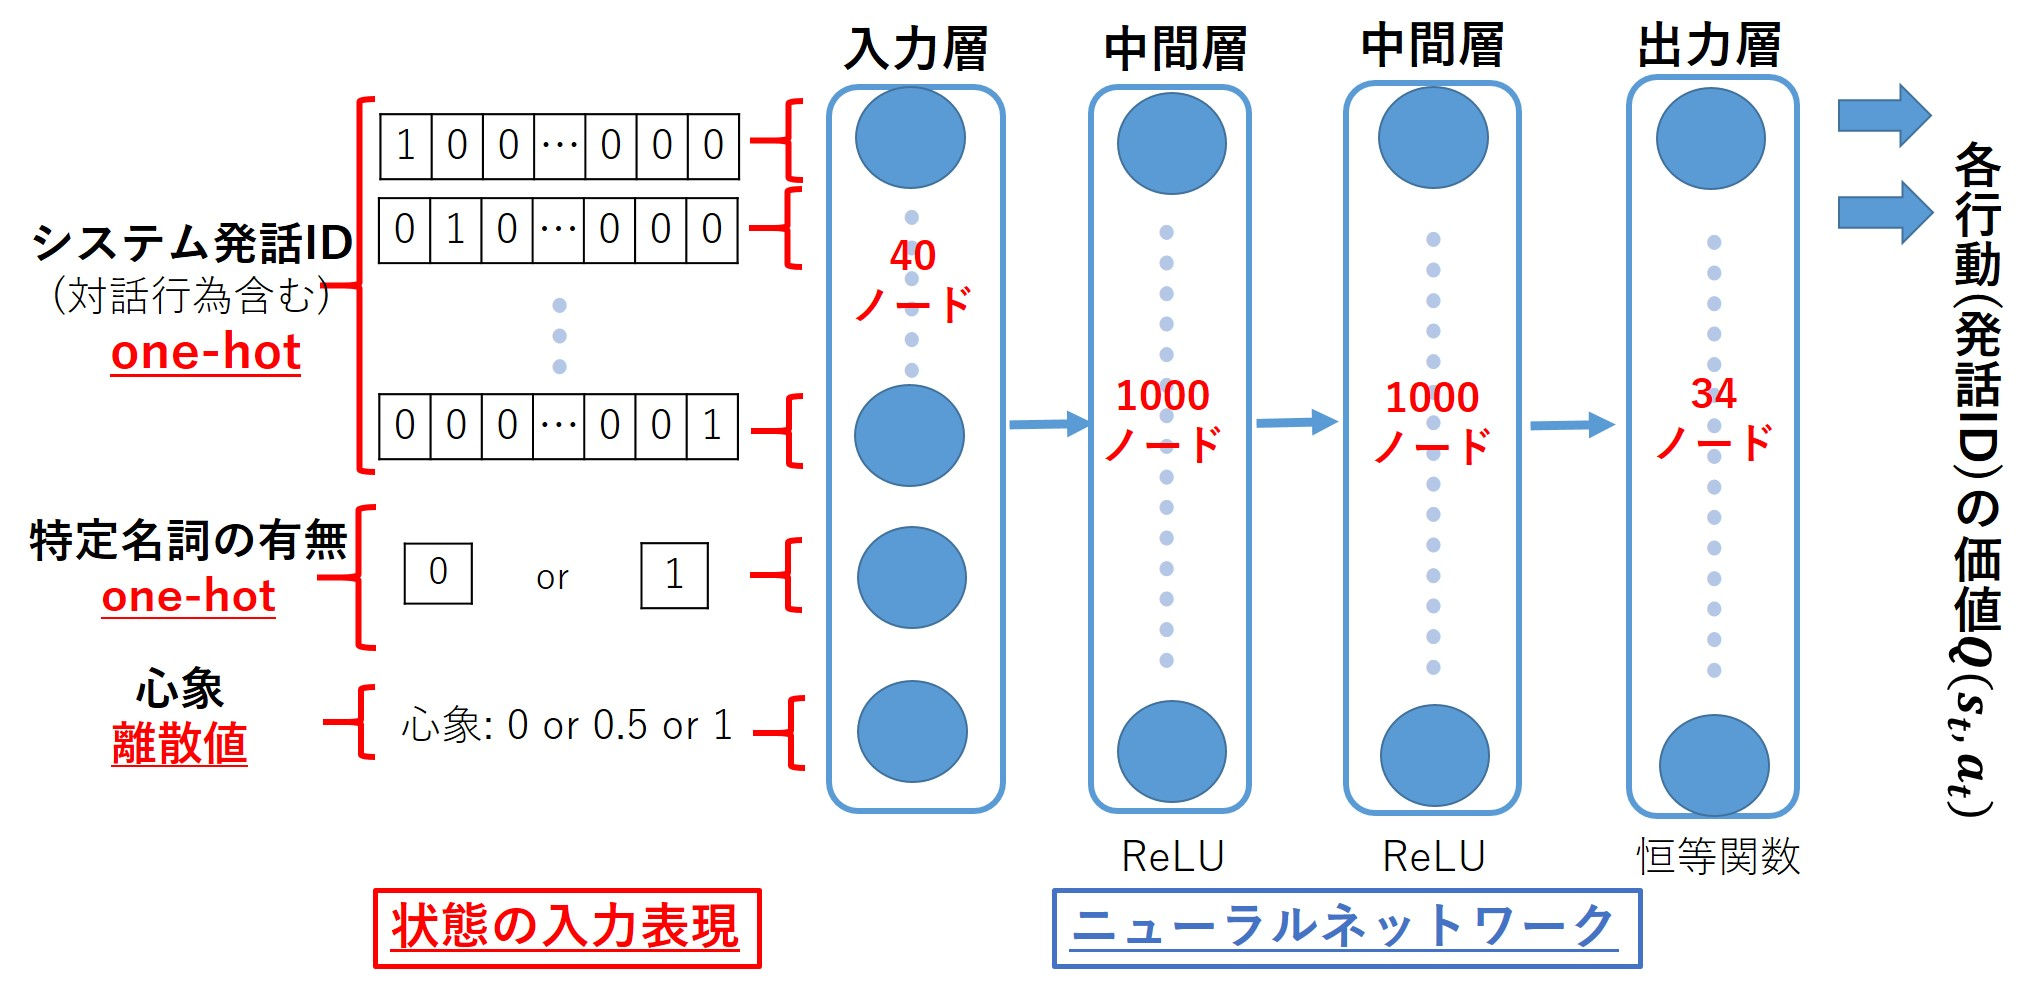
\includegraphics[width=12cm]{input_NN_re2.jpg}
    \caption{DQNを用いる場合の設計}
    \label{input_NN}
\end{figure*}

\subsection{Deep Q Network}
Deep Q Networkとは,Q学習ではテーブル形式で表現されていた行動価値関数を,ニューラルネットによって関数近似したものである.
Q学習では全状態に関してQ値を更新しなければならないが,
そのため,DQNではQ学習に比べて多くの状態を扱うことができる.

DQNで学習されたニューラルネットワークは,Q学習における状態を入力とし,その状態における各行動のQ値を出力する.
ニューラルネットワークの学習方法としては,損失関数を最小化するように重みを調整する.ここでの損失関数は,あるターン$t$での状態$s_{t}$,行動$a_{t}$と,次のターン$t+1$での状態$s_{t+1}$,報酬$r_{t+1}$,また,学習率$\alpha$,割引率$\gamma$を用いて式\ref{DQN}のように表される.
\begin{equation}
\label{DQN}
E(s_t,a_t) = (r_{t+1}+\gamma*max_aQ(s_{t+1},a)-Q(s_t,a_t))^2
\end{equation}
また,DQNの学習安定のために以下のような工夫がある.
\begin{description}
   \item[Experience replay]\mbox{}\\
   Q学習では各ステップごとに学習を行っていたが,ニューラルネットワークを用いる場合,時間的に相関が高い内容を学習してしまい,過学習が起きやすい.
   そこで,状態,行動,報酬,次の状態を各ステップごとにメモリに蓄積していき,ランダムにサンプリングしてから学習する.
   \item[Target Q Network]\mbox{}\\%式\ref{DQN}の$max_aQ(s_(s+1),a)$つまり次の状態の最大のQ値を用いる際,
   ニューラルネットワークの更新には式\ref{DQN}の損失関数が用いられるが,式内のQ値の計算に毎回更新した直後のニューラルネットワークを用いると学習が安定しない.そのため,Q値の計算に用いるニューラルネットワークはしばらくの間固定し,一定間隔で更新していく形を取る.
\end{description}
\subsection{入力表現}%発話IDをIDのまま入力した場合
DQNを適用する際には,Q学習における状態をニューラルネットワークで扱える形にする必要がある.
具体的には,\ref{Qlearning_sekkei}章で示した4種の状態をニューラルネットワークの入力表現にする.

まず,「システム発話の対話行為」に関しては,システム発話IDがより細かく分類したものにあたるため,考慮しない.

次に,「ユーザ発話内の特定名詞の有無」に関しては,2値を取るため0 or 1で表現した.

また,「ユーザ心象」に関しては,低,中,高の3段階に離散化し,それぞれに0, 0.5, 1の数値を割り当てた.

「システム発話ID」の表現方法を決定する際には,発話ID(1〜38)を正規化して用いる方法と,ID数分の長さのone$-$hotベクトルを用意し,該当IDの発話が現れたときに1をたてる方法の両方を試した.
この結果を縦軸が行動に番号を振ったもの,横軸が状態の組み合わせに番号を振ったものである,Qテーブルのヒートマップ図\ref{hyogen1},\ref{hyogen2}に示す.

結果として,図\ref{hyogen1}のように,IDを正規化して用いる方法ではほとんどの状態で行動価値が同じになってしまい,適切に学習できているとは言えない.
一方,one$-$hotベクトルを用いる方法では,図\ref{hyogen2}ように,状態ごとの行動価値に適度なばらつきが見られる.
これはID化された発話間に数学的に連続な関係がないことが原因であると考えられる.

この結果から,「システム発話ID」の入力表現にはone$-$hotベクトルを用いる方法を採用した.
\begin{figure*}[tb]
 \begin{minipage}{0.45\hsize}
  \begin{center}
   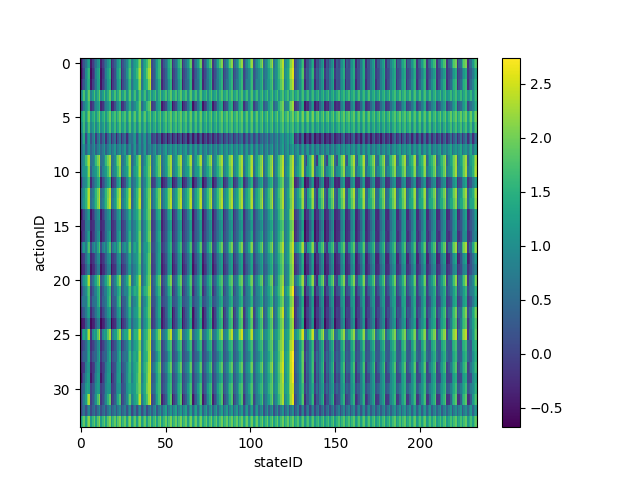
\includegraphics[width=\linewidth]{table_hyogen.png}
  \end{center}
  \caption{発話IDを正規化して用いた時のQテーブル}
  \label{hyogen1}
 \end{minipage}
 \begin{minipage}{0.45\hsize}
  \begin{center}
   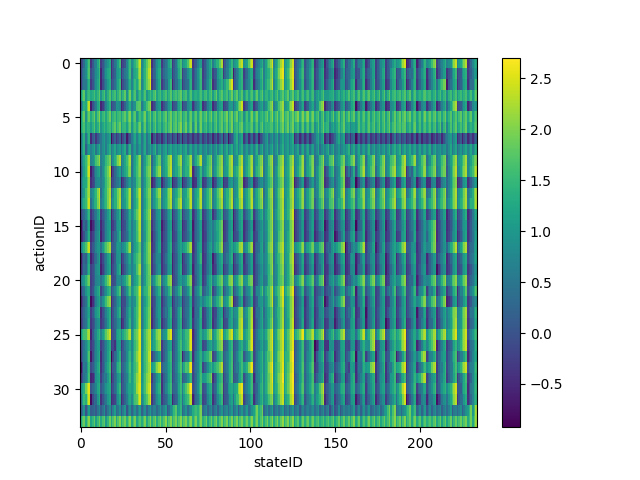
\includegraphics[width=\linewidth]{table_DQN.png}
  \end{center}
  \caption{one$-$hotベクトル用いた時のQテーブル}
  \label{hyogen2}
 \end{minipage}
\end{figure*}

%\subsection{報酬の正規化}%報酬を正規化しなかった場合
%DQNの報酬に関しては,値が大きすぎるとニューラルネットワークの学習が安定しない.
%そのため,Q学習に用いていた報酬を正規化し,新たな報酬として与えることで学習の安定化を図った.
\subsection{中間層のノード数の設定}%中間層ノード数を変えてみた場合
中間層のノード数を決定する際には,1,5,10,100,1000と変え,Qテーブルの変化を見ながら値を選んだ.
この結果を,縦軸が行動に番号を振ったもの,横軸が状態の組み合わせに番号を振ったものである,Qテーブルのヒートマップ図\ref{tyukanso}に示す.
図\ref{tyukanso}を見ると,中間層のノード数が1や5と小さいときには,異なる状態でも同じような行動の価値が高くなっている.
一方,10,100,1000とノード数を増やしていくと,徐々に状態ごとの行動価値にばらつきが現れ,100〜1000程度で安定した.
これは中間層のノード数を増やすごとに,ニューラルネットワークの表現力が上がっているためと考えられる.

この結果から,中間層のノード数は1000とした.

\begin{figure*}[htb]
    \centering
    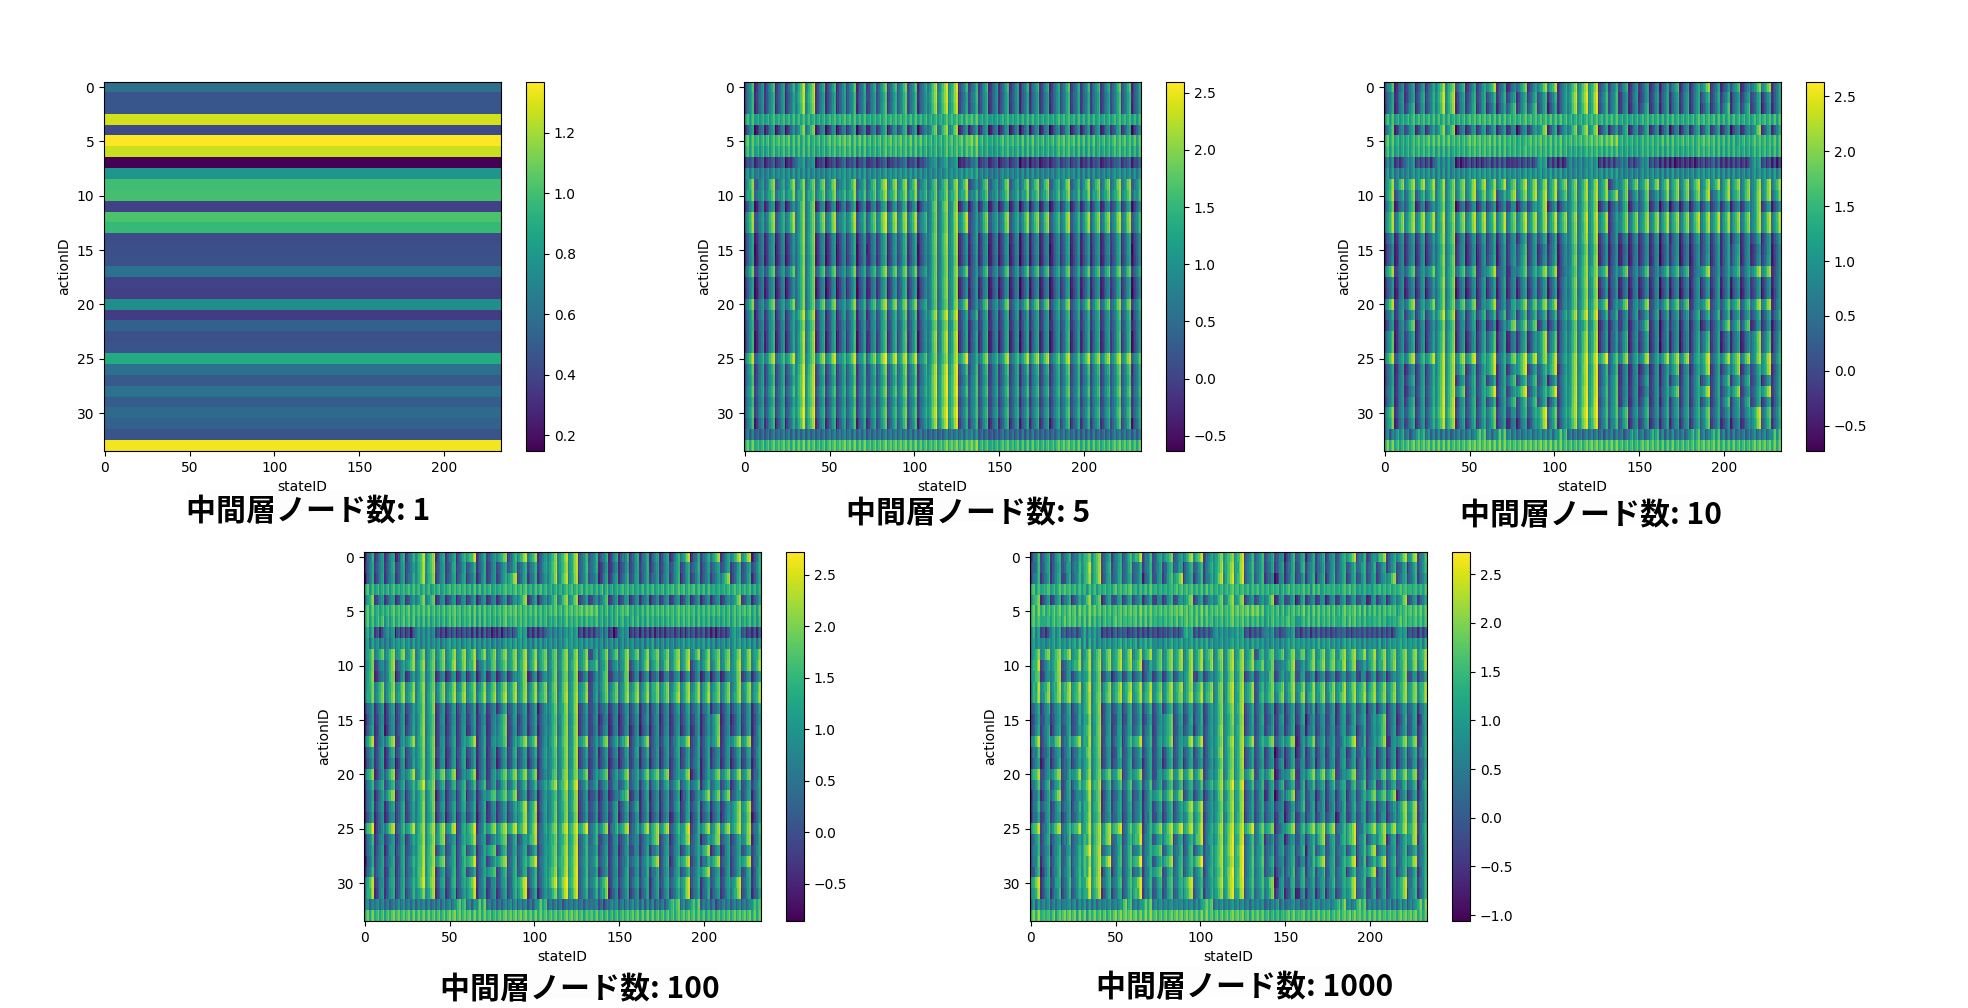
\includegraphics[width=\hsize]{tyukanso.jpg}
    \caption{DQNにおける中間層ノード数ごとのQテーブル}
    \label{tyukanso}
\end{figure*}


\section{Q学習による実装とDQNによる実装の比較}
本章では,システム発話間の整合性を重視した発話選択の学習方法として,Q学習を用いた場合と,DQNを用いた場合の比較を行う.

まず,学習過程における違いを調べると,十分に学習できるまでにかかるエピソード数に違いがあったたため,その回数を報告する.

次に,両者のQテーブルを見比べ,今回実装したDQNによる手法でQ学習を用いた場合と同様の学習ができているかを調べる.
また,実際に対話を行い,不適切な発話が選択される数をカウントすることで,システム発話間の整合性を重視した手法の再現ができていることを確かめる.



\subsection{実験条件}
システム発話のデータは雑談対話コーパスHazumi1902\cite{Hazumi}収集時に使用された発話から,
「スポーツ」,「音楽」,「食事」,「旅行」の話題にラベル付けされたものを用いた.
具体的には,それぞれの話題の発話集合に,どの話題でも用いることのできる「default」発話を加えた発話集合を作成し,4つそれぞれに関してQテーブルを学習した.発話集合はいずれも60〜70発話で構成されている.

Q学習で十分な学習を行うためには,膨大な数の対話サンプルが必要となる.しかし,そのような対話サンプルを実際に収集するのは現実的ではない.そのため,システム発話に対応するユーザ発話とユーザ心象を出力するようなユーザモデルを用いた.具体的には,ユーザモデルはシステム発話に対して,コーパス収集時と同じ発話を返す.

学習時の行動選択方策としては,確率epsilonでランダムな行動選択をし,それ以外でQ値が最大となる行動選択をするepsilon greedy法を用いた.
強化学習においては,学習の初期フェイズではランダムな探索を多く行い,十分な探索が行えたら学習結果を用いた行動選択によってQ値の安定を図るのが望ましい.そこで,今回の実装では,epsilonを初期値1,終値0.1として全体のエピソード数の1/4の学習を終えるまで減衰させ続けた.
現在のエピソード数をc\_e(current\_episode),全体のエピソード数をe(episode)とすると,epsilonは式\ref{epsilon}のように表される.
\begin{equation}\label{epsilon}\begin{split}&epsilon=max(1-0.9*c\_e*(\frac{e}{4}),0.1)\end{split}\end{equation}

学習エピソード数は,10交換の対話を1エピソードとし,それぞれの手法において,十分に学習されるまでとした.
強化学習において,十分に学習されたと判断されるタイミングは,得られる報酬の平均が変化しなくなった時である.
しかし,学習の初期フェイズでランダム探索が十分でない場合,報酬の平均が低い値で安定してしまうことがある.
そこで,本稿では報酬の平均が変化しなくなるエピソード数を検証し,それを十分な学習に必要なエピソード数とした.

\subsection{十分な学習に必要なエピソード数の比較}
十分な学習に必要なエピソード数を検証する際,Q学習とDQNで明らかな差が生じた.
図\ref{hosyu_suii_re}にそれぞれの手法において,平均報酬が変化しなくなった時のエピソードごとの報酬推移を示す.
結果として,Q学習では500000回,DQNでは50000回学習させたところで報酬平均の変化が止まった.

このことから,DQNを用いた手法では,Q学習より少ないエピソード数で十分な学習が行えることがわかる.
%この原因として

\subsection{Qテーブルによる比較}
Qテーブルを比較することでDQNを用いた実装で,Q学習を用いた手法の再現ができているか調べた.
ただし,DQNのQ関数はニューラルネットであるため,一旦状態に対応するQ値をニューラルネットから出力し,テーブル形式に直して比較した.

比較した結果として,同様のQテーブルが得られていることを確認した.
\subsection{対話による比較}
話題「スポーツ」に関して10交換の対話を10セットずつ行い,Q学習を用いた手法とDQNを用いた手法の不適切な発話が選択される数をカウントした.
ここで,適切な発話と不適切な発話の例を図\ref{tekihuteki}に示す.
不適切な発話とは例のように,選択したシステム発話に違和感が感じられるような場合である.


結果は表\ref{hikaku_taiwa}のようにほぼ同数であり,不適切な発話を防ぐという点で同等の性能を再現できていることがわかる.





\begin{table}[tb]
\caption{対話における不適切な発話選択の数}
\centering
  \begin{tabular}{|l|c|c|c|} \hline
      &適切& 不適切 \\ \hline \hline
    Q学習を用いたシステム & 94 & 6 \\ \hline
    DQNを用いたシステム & 95 & 5  \\ \hline
  \end{tabular}\label{hikaku_taiwa}
\end{table}


\begin{figure*}[tb]
    \centering
    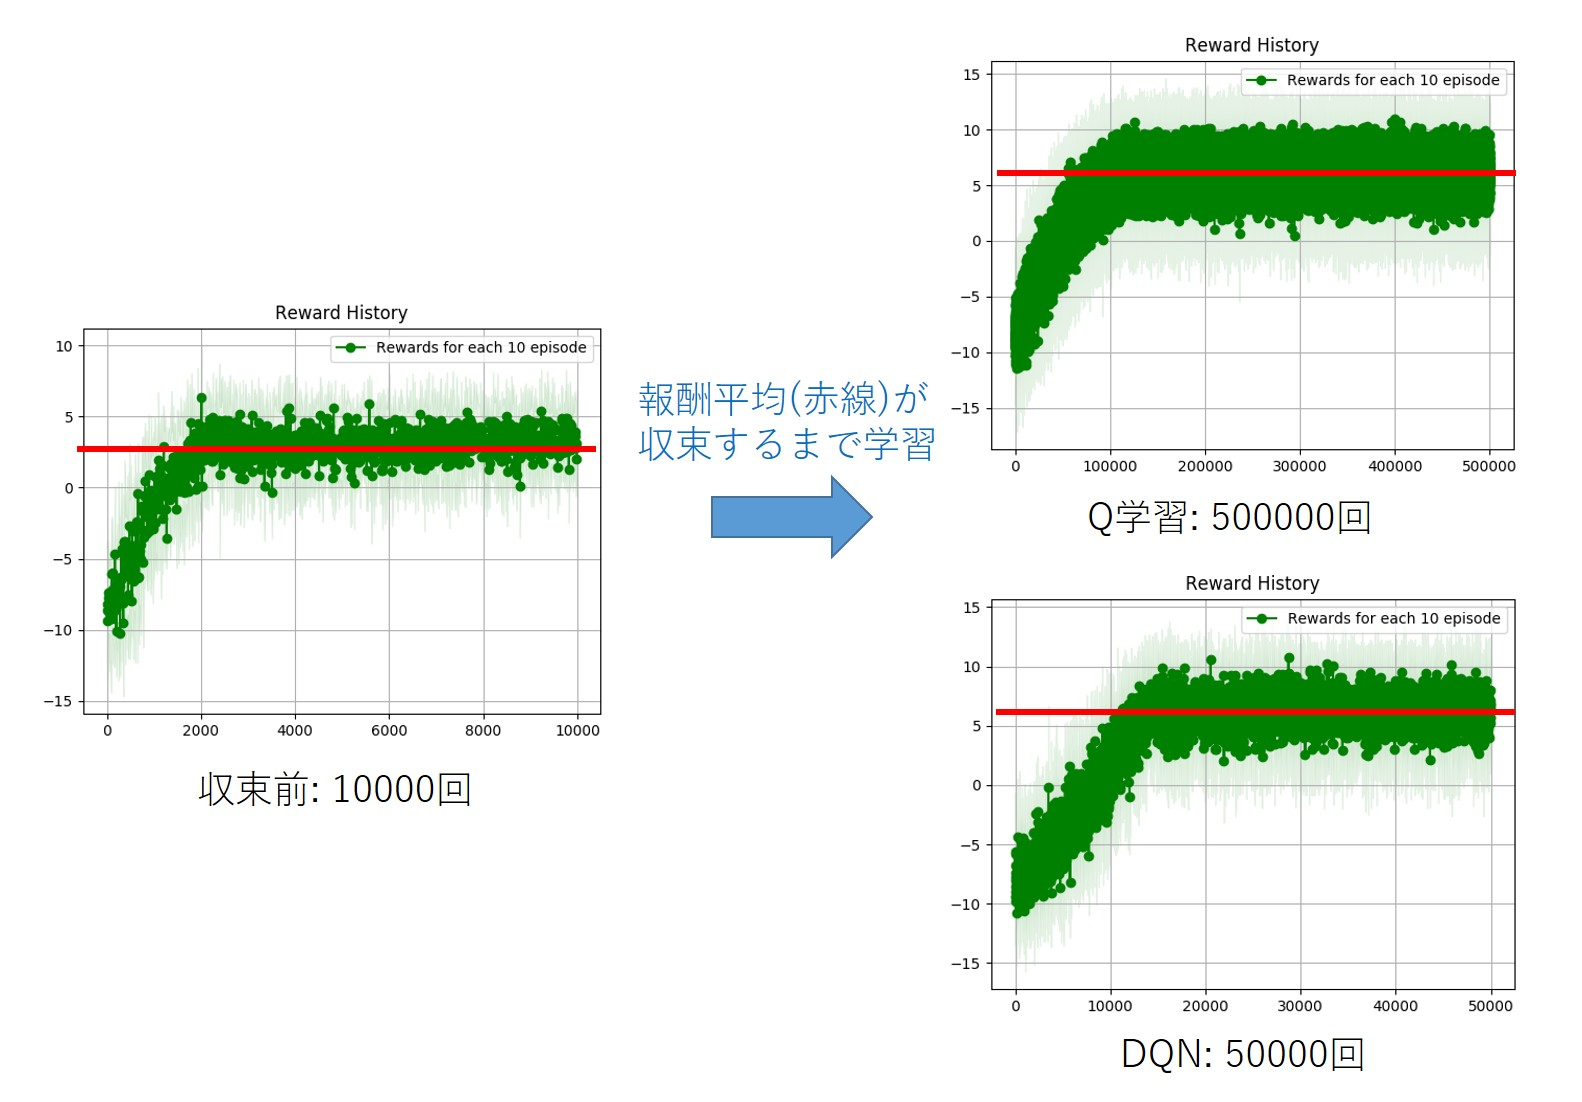
\includegraphics[width=0.8\hsize]{hosyusuii_re.jpg}
    \caption{Q学習とDQNにおける報酬平均の収束}
    \label{hosyu_suii_re}
\end{figure*}


\begin{figure}[tb]
\centering
%\small
%\begin{Verbatim}[commandchars=\\\{\}]


\begin{Verbatim}[commandchars=\\\{\}]
【不適切】
S: 競技は何をご覧になりますか?
U: 野球です
\mychangecolor{S: それは大変ですよね}
U: 大変ですかね
\end{Verbatim}
%\caption{破綻パターン2}
%\label{hatan2}

\begin{Verbatim}[commandchars=\\\{\}]
【適切】
S: 競技は何をご覧になりますか?
U: 野球です
\mychangecolor{S: それは面白そうですね}
U: ええとても面白いです
\end{Verbatim}


\caption{不適切な発話選択と適切な発話選択の例(赤字)}
\label{tekihuteki}
\end{figure}
%%%%%%%%%%%%%%%%%%%%%%%%%%%%%%%%%%%%%%

\section{おわりに}
本稿では,聞き役対話システムの発話選択の強化学習による定式化において,将来的により多くの状態を考慮できるように,DQNの枠組みの導入を目指した.以前Q学習を用いて実装したシステム発話間の整合性を重視した発話選択を,DQNを用いて再現することにより,入力表現や報酬の扱い,パラメータの設定などに関して,当該タスクへのDQNの適用方法の知見を得た.
また,Q学習の場合と学習過程を比較することで,より少ないエピソード数で十分な学習が行えることを確かめた.

\bibliography{name} %hoge.bibから拡張子を外した名前
\bibliographystyle{junsrt} %参考文献出力スタイル
\end{document}

